\documentclass[a4]{article}

% PAQUETES %%%%%%%%%%%%%%%%%%%%%%%%%%%%%%%%%%%%%%%%%%%%%%%%%%%%%%%%%%%%%%%%%%%%%
\usepackage[utf8]{inputenc}
\usepackage{framed} % Para crear cuadros alrededor del texto
\usepackage{makecell}
\usepackage[english]{babel}
%
\usepackage[fixlanguage]{babelbib}
    \bibliographystyle{IEEEtran}

\usepackage{url}

%!TEX encoding = UTF-8 Unicode
% !TEX spellcheck = es

\setlength{\textwidth}{6.5 in}
\setlength{\textheight}{8.5 in}
\setlength{\headsep}{0.5 in}

\usepackage{multirow, array} % para las tablas
\usepackage{float} % para usar [H]
\usepackage{charter}

\usepackage[breaklinks=true]{hyperref}

%
% ADD PACKAGES here:
%

\usepackage[utf8]{inputenc}
\usepackage{amsmath,longtable,siunitx, float, graphicx, dcolumn, bm, fancyhdr, authblk, subcaption, caption, hyperref, multicol, setspace}

\usepackage{bbding}
\usepackage{amssymb}
\usepackage[rightcaption]{sidecap}
%\usepackage{textcomp}

\usepackage[hmarginratio=1:1, top=32mm, columnsep=20pt, headsep=\dimexpr20mm, margin=0.7in, top=1in ]{geometry}

\usepackage{booktabs}
\usepackage{multirow}

\usepackage{algorithm}
\usepackage{enumitem}
\usepackage{tabularx}
\usepackage[noend]{algpseudocode}
\usepackage{xcolor}

\usepackage{tikz}
\usetikzlibrary{shapes.geometric, arrows.meta, positioning}

% ----------- global styles -----------
\tikzset{
  font=\scriptsize,                      % tiny text everywhere
  every node/.style       = {transform shape},   % respect scale
  startstop/.style        = {ellipse, draw, fill=blue!10,
                             inner sep=1pt, minimum width=13mm},
  process/.style          = {rectangle, draw, fill=orange!15,
                             text width=26mm, inner sep=2pt, align=center},
  decision/.style         = {diamond, draw, fill=green!15, aspect=2.3,
                             text width=20mm, inner sep=1pt, align=center},
  arrow/.style            = {->, >=Stealth, shorten >=1pt, shorten <=1pt}
}

\newcommand{\TODO}{\textbf{\textcolor{red}{TODO}}}

\renewcommand{\algorithmicrequire}{\textbf{Input:}}
\renewcommand{\algorithmicensure}{\textbf{Output:}}

\lhead{\includegraphics[scale=0.4]{CETC.png}}
\rhead{\includegraphics[scale=0.025]{Cornell-University-Logo.png}}

\newtheorem{theo}{Theorem}
\newenvironment{theorem}
  {\begin{mdframed}\begin{theo}}
  {\end{theo}\end{mdframed}}

\newtheorem{prop}{Proposición}
\newenvironment{proposition}
  {\begin{mdframed}\begin{prop}}
  {\end{prop}\end{mdframed}}

\newtheorem{lem}{Lema}
\newenvironment{lema}
  {\begin{mdframed}\begin{lem}}
  {\end{lem}\end{mdframed}}

\newtheorem{defi}{Definition}
\newenvironment{definition}
  {\begin{mdframed}\begin{def}}
  {\end{def}\end{mdframed}}

\newtheorem{proof}{Proof}
\newtheorem{remark}{Remark}

\usepackage[numbers]{natbib}
\renewcommand{\thesection}{\Roman{section}}
%\setlength{\parskip}{\baselineskip}%

\begin{document}

\thispagestyle{fancy}

\begin{center}
    \textbf{\large Orbit Odyssey - Computer Vision} \\
    {Field Definition --- All Layouts}

    \vspace{0.7em}

    David Alejandro Fuquen \\

    {\small \today}

\end{center}

\section*{Compilation of Field Definitions}

\subsection*{Summary}

This document consolidates all six available field layouts for the Orbit Odyssey Computer Vision Challenge into a single reference. Each layout defines the object positions, clearance constraints, and class rotation templates for a specific field configuration.

The six layouts fall into three categories:

\begin{itemize}
    \item \textbf{No-partition, corner start:} NP\_5 (5 objects, diamond) and NP\_6 (6 objects, staggered 2$\times$3).
    \item \textbf{Partition, corner start:} P\_5 (5 objects, zigzag 3+2) and P\_6 (6 objects, zigzag 3+3).
    \item \textbf{Center-start fallback:} NP\_4 (3 objects, no partition) and P\_3 (3 objects, partition). Use only if \texttt{main.py} cannot be modified for corner starts.
\end{itemize}

\subsection*{Shared field specifications}

All layouts share the following field dimensions and rules.

\begin{table}[H]
\centering
\begin{tabular}{ll}
\toprule
\textbf{Property} & \textbf{Value} \\
\midrule
Total length (X-axis) & 254.00 cm (100 in) \\
Total width (Y-axis) & 142.24 cm (56 in) \\
Total floor area & 3.61 m\textsuperscript{2} \\
Perimeter walls & Low-profile PVC pipe barriers \\
Corner zones (Low Rubble Zones) & 30.48 $\times$ 30.48 cm (12 $\times$ 12 in) at each corner \\
Object approximate radius & 6 cm \\
\bottomrule
\end{tabular}
\caption{Shared field dimensions.}
\end{table}

The coordinate system places the origin $(0, 0)$ at the bottom-left corner of the field. The X-axis runs left to right (0 to 254 cm) and the Y-axis runs bottom to top (0 to 142.24 cm).

\subsubsection*{Central partition (P\_5, P\_6, P\_3 only)}

\begin{table}[H]
\centering
\begin{tabular}{ll}
\toprule
\textbf{Property} & \textbf{Value} \\
\midrule
Orientation & Horizontal, centered on both axes \\
Y-axis position & Y = 71.12 cm (28 in) --- midpoint of field width \\
Length & 127.00 cm (50 in) --- half the field length \\
X-axis span & X = 63.50 cm to X = 190.50 cm \\
Left gap & X = 0 to 63.50 cm (25 in wide) \\
Right gap & X = 190.50 to 254.00 cm (25 in wide) \\
Height & Same as perimeter walls (camera sees over it) \\
\bottomrule
\end{tabular}
\caption{Central partition specifications.}
\end{table}

\subsubsection*{Clearance rules}

\begin{itemize}
    \item Object center to wall $\geq$ 20 cm.
    \item Object center to object center $\geq$ 35 cm.
    \item Object center to partition $\geq$ 20 cm (partition layouts only).
    \item No object may be placed inside a corner zone.
\end{itemize}

\subsection*{Layout comparison}

\begin{table}[H]
\centering
\begin{tabular}{llccll}
\toprule
\textbf{Layout} & \textbf{Partition} & \textbf{Objects} & \textbf{Classes} & \textbf{Start} & \textbf{Pattern} \\
\midrule
NP\_5 & No & 5 & 1R + 2T + 2TC & Corner & Diamond with center \\
NP\_6 & No & 6 & 2R + 2T + 2TC & Corner & Staggered 2$\times$3 \\
P\_5 & Yes & 5 & 1R + 2T + 2TC & Corner & Zigzag (3 bottom, 2 top) \\
P\_6 & Yes & 6 & 2R + 2T + 2TC & Corner & Zigzag (3 bottom, 3 top) \\
NP\_4 & No & 3 & 1R + 1T + 1TC & Center & Equilateral triangle \\
P\_3 & Yes & 3 & 1R + 1T + 1TC & Center (bottom) & Triangle above robot \\
\bottomrule
\end{tabular}
\caption{Layout comparison. R = Rocket, T = Tire, TC = Tin Can.}
\end{table}

%% ============================================================
%% LAYOUT 1: NP_5
%% ============================================================
\pagebreak
\section*{Layout 1: NP\_5 --- Diamond with Center Point}

\textbf{No partition. 5 objects. Corner start.}

This layout uses \textbf{5 objects}: 1 Rocket + 2 Tires + 2 Tin Cans, arranged in a diamond pattern with a center point. The layout is perfectly symmetric --- no corner has an advantage.

\begin{figure}[H]
\centering
\begin{tikzpicture}
  \begin{scope}[scale=0.055]
    \draw[thick] (0,0) rectangle (254, 142.24);
    \draw[dashed, blue!60] (0,0) rectangle (30.48, 30.48);
    \draw[dashed, blue!60] (254-30.48,0) rectangle (254, 30.48);
    \draw[dashed, blue!60] (0,142.24-30.48) rectangle (30.48, 142.24);
    \draw[dashed, blue!60] (254-30.48,142.24-30.48) rectangle (254, 142.24);
    \filldraw[red!70!black] (63.50, 35.56) circle (6);
    \filldraw[red!70!black] (190.50, 35.56) circle (6);
    \filldraw[red!70!black] (127.00, 71.12) circle (6);
    \filldraw[red!70!black] (63.50, 106.68) circle (6);
    \filldraw[red!70!black] (190.50, 106.68) circle (6);
    \draw[dashed, gray!50] (63.50,35.56) -- (127.00,71.12) -- (190.50,35.56);
    \draw[dashed, gray!50] (63.50,106.68) -- (127.00,71.12) -- (190.50,106.68);
    \draw[dashed, gray!50] (63.50,35.56) -- (63.50,106.68);
    \draw[dashed, gray!50] (190.50,35.56) -- (190.50,106.68);
    \draw[<->, >=Stealth] (0,-12) -- (254,-12);
    \draw[<->, >=Stealth] (-12,0) -- (-12,142.24);
  \end{scope}
  \node[font=\footnotesize\bfseries, anchor=north] at (3.49,1.63) {\textsf{P1}};
  \node[font=\footnotesize\bfseries, anchor=north] at (10.48,1.63) {\textsf{P2}};
  \node[font=\footnotesize\bfseries, anchor=west] at (7.35,3.91) {\textsf{P3}};
  \node[font=\footnotesize\bfseries, anchor=south] at (3.49,6.20) {\textsf{P4}};
  \node[font=\footnotesize\bfseries, anchor=south] at (10.48,6.20) {\textsf{P5}};
  \node[blue!70, font=\scriptsize] at (0.84,0.84) {LRZ};
  \node[blue!70, font=\scriptsize] at (13.13,0.84) {LRZ};
  \node[blue!70, font=\scriptsize] at (0.84,6.98) {LRZ};
  \node[blue!70, font=\scriptsize] at (13.13,6.98) {LRZ};
  \node[font=\footnotesize] at (6.99,-1.10) {254 cm (100 in)};
  \node[font=\footnotesize, rotate=90] at (-1.21,3.91) {142.24 cm (56 in)};
  \node[font=\scriptsize, anchor=north east] at (-0.11,-0.11) {$(0,0)$};
\end{tikzpicture}
\caption{Layout NP\_5 --- diamond pattern with center point (no partition).}
\end{figure}

\subsection*{Object positions}

\begin{table}[H]
\centering
\begin{tabular}{clcccc}
\toprule
\textbf{ID} & \textbf{Location} & \textbf{X (in)} & \textbf{Y (in)} & \textbf{X (cm)} & \textbf{Y (cm)} \\
\midrule
P1 & Bottom-left quadrant & 25 & 14 & 63.50 & 35.56 \\
P2 & Bottom-right quadrant & 75 & 14 & 190.50 & 35.56 \\
P3 & Dead center & 50 & 28 & 127.00 & 71.12 \\
P4 & Top-left quadrant & 25 & 42 & 63.50 & 106.68 \\
P5 & Top-right quadrant & 75 & 42 & 190.50 & 106.68 \\
\bottomrule
\end{tabular}
\caption{Object positions --- NP\_5.}
\end{table}

\subsection*{Clearance verification}

\begin{table}[H]
\centering
\begin{tabular}{ccccccc}
\toprule
\textbf{ID} & \textbf{Left wall} & \textbf{Right wall} & \textbf{Bottom wall} & \textbf{Top wall} & \textbf{Min wall} & \textbf{Nearest obj.} \\
\midrule
P1 & 63.5 & 190.5 & 35.6 & 106.7 & 35.6 \checkmark & 71.1 (P4) \checkmark \\
P2 & 190.5 & 63.5 & 35.6 & 106.7 & 35.6 \checkmark & 71.1 (P5) \checkmark \\
P3 & 127.0 & 127.0 & 71.1 & 71.1 & 71.1 \checkmark & 72.8 (P1) \checkmark \\
P4 & 63.5 & 190.5 & 106.7 & 35.6 & 35.6 \checkmark & 71.1 (P1) \checkmark \\
P5 & 190.5 & 63.5 & 106.7 & 35.6 & 35.6 \checkmark & 71.1 (P2) \checkmark \\
\bottomrule
\end{tabular}
\caption{Clearance verification --- NP\_5 (all values in cm).}
\end{table}

\subsection*{Distance from each corner to each object (cm)}

\begin{table}[H]
\centering
\begin{tabular}{lccccc}
\toprule
\textbf{Corner} & \textbf{P1} & \textbf{P2} & \textbf{P3} & \textbf{P4} & \textbf{P5} \\
\midrule
Bottom-Left & \textbf{52} & 176 & 125 & 103 & 198 \\
Bottom-Right & 176 & \textbf{52} & 125 & 198 & 103 \\
Top-Left & 103 & 198 & 125 & \textbf{52} & 176 \\
Top-Right & 198 & 103 & 125 & 176 & \textbf{52} \\
\bottomrule
\end{tabular}
\caption{Corner distances --- NP\_5.}
\end{table}

\subsection*{Class rotation templates}

\begin{table}[H]
\centering
\begin{tabular}{lccccc}
\toprule
\textbf{Template} & \textbf{P1} & \textbf{P2} & \textbf{P3} & \textbf{P4} & \textbf{P5} \\
\midrule
A & Rocket & Tire & Tin Can & Tire & Tin Can \\
B & Tin Can & Rocket & Tire & Tin Can & Tire \\
C & Tire & Tin Can & Rocket & Tin Can & Tire \\
D & Tire & Tin Can & Tin Can & Rocket & Tire \\
\bottomrule
\end{tabular}
\caption{Rotation templates --- NP\_5.}
\end{table}

%% ============================================================
%% LAYOUT 2: NP_6
%% ============================================================
\pagebreak
\section*{Layout 2: NP\_6 --- Staggered 2$\times$3}

\textbf{No partition. 6 objects. Corner start.}

This layout uses \textbf{6 objects}: 2 Rockets + 2 Tires + 2 Tin Cans, arranged in a staggered 2$\times$3 pattern with a slight hexagonal offset between rows. The layout is symmetric --- no corner has an advantage.

\begin{figure}[H]
\centering
\begin{tikzpicture}
  \begin{scope}[scale=0.055]
    \draw[thick] (0,0) rectangle (254, 142.24);
    \draw[dashed, blue!60] (0,0) rectangle (30.48, 30.48);
    \draw[dashed, blue!60] (254-30.48,0) rectangle (254, 30.48);
    \draw[dashed, blue!60] (0,142.24-30.48) rectangle (30.48, 142.24);
    \draw[dashed, blue!60] (254-30.48,142.24-30.48) rectangle (254, 142.24);
    \filldraw[red!70!black] (55.88, 40.64) circle (6);
    \filldraw[red!70!black] (127.00, 35.56) circle (6);
    \filldraw[red!70!black] (198.12, 40.64) circle (6);
    \filldraw[red!70!black] (55.88, 101.60) circle (6);
    \filldraw[red!70!black] (127.00, 106.68) circle (6);
    \filldraw[red!70!black] (198.12, 101.60) circle (6);
    \draw[dashed, gray!50] (55.88,40.64) -- (127.00,35.56) -- (198.12,40.64);
    \draw[dashed, gray!50] (55.88,101.60) -- (127.00,106.68) -- (198.12,101.60);
    \draw[dashed, gray!50] (55.88,40.64) -- (55.88,101.60);
    \draw[dashed, gray!50] (127.00,35.56) -- (127.00,106.68);
    \draw[dashed, gray!50] (198.12,40.64) -- (198.12,101.60);
    \draw[<->, >=Stealth] (0,-12) -- (254,-12);
    \draw[<->, >=Stealth] (-12,0) -- (-12,142.24);
  \end{scope}
  \node[font=\footnotesize\bfseries, anchor=north] at (3.07,1.90) {\textsf{P1}};
  \node[font=\footnotesize\bfseries, anchor=north] at (6.99,1.62) {\textsf{P2}};
  \node[font=\footnotesize\bfseries, anchor=north] at (10.90,1.90) {\textsf{P3}};
  \node[font=\footnotesize\bfseries, anchor=south] at (3.07,5.92) {\textsf{P4}};
  \node[font=\footnotesize\bfseries, anchor=south] at (6.99,6.20) {\textsf{P5}};
  \node[font=\footnotesize\bfseries, anchor=south] at (10.90,5.92) {\textsf{P6}};
  \node[blue!70, font=\scriptsize] at (0.84,0.84) {LRZ};
  \node[blue!70, font=\scriptsize] at (13.13,0.84) {LRZ};
  \node[blue!70, font=\scriptsize] at (0.84,6.98) {LRZ};
  \node[blue!70, font=\scriptsize] at (13.13,6.98) {LRZ};
  \node[font=\footnotesize] at (6.99,-1.10) {254 cm (100 in)};
  \node[font=\footnotesize, rotate=90] at (-1.21,3.91) {142.24 cm (56 in)};
  \node[font=\scriptsize, anchor=north east] at (-0.11,-0.11) {$(0,0)$};
\end{tikzpicture}
\caption{Layout NP\_6 --- staggered 2$\times$3 pattern (no partition).}
\end{figure}

\subsection*{Object positions}

\begin{table}[H]
\centering
\begin{tabular}{clcccc}
\toprule
\textbf{ID} & \textbf{Location} & \textbf{X (in)} & \textbf{Y (in)} & \textbf{X (cm)} & \textbf{Y (cm)} \\
\midrule
P1 & Bottom-left & 22 & 16 & 55.88 & 40.64 \\
P2 & Bottom-center & 50 & 14 & 127.00 & 35.56 \\
P3 & Bottom-right & 78 & 16 & 198.12 & 40.64 \\
P4 & Top-left & 22 & 40 & 55.88 & 101.60 \\
P5 & Top-center & 50 & 42 & 127.00 & 106.68 \\
P6 & Top-right & 78 & 40 & 198.12 & 101.60 \\
\bottomrule
\end{tabular}
\caption{Object positions --- NP\_6.}
\end{table}

\subsection*{Clearance verification}

\begin{table}[H]
\centering
\begin{tabular}{ccccccc}
\toprule
\textbf{ID} & \textbf{Left wall} & \textbf{Right wall} & \textbf{Bottom wall} & \textbf{Top wall} & \textbf{Min wall} & \textbf{Nearest obj.} \\
\midrule
P1 & 55.9 & 198.1 & 40.6 & 101.6 & 40.6 \checkmark & 61.0 (P4) \checkmark \\
P2 & 127.0 & 127.0 & 35.6 & 106.7 & 35.6 \checkmark & 71.1 (P5) \checkmark \\
P3 & 198.1 & 55.9 & 40.6 & 101.6 & 40.6 \checkmark & 61.0 (P6) \checkmark \\
P4 & 55.9 & 198.1 & 101.6 & 40.6 & 40.6 \checkmark & 61.0 (P1) \checkmark \\
P5 & 127.0 & 127.0 & 106.7 & 35.6 & 35.6 \checkmark & 71.1 (P2) \checkmark \\
P6 & 198.1 & 55.9 & 101.6 & 40.6 & 40.6 \checkmark & 61.0 (P3) \checkmark \\
\bottomrule
\end{tabular}
\caption{Clearance verification --- NP\_6 (all values in cm).}
\end{table}

\subsection*{Distance from each corner to each object (cm)}

\begin{table}[H]
\centering
\begin{tabular}{lcccccc}
\toprule
\textbf{Corner} & \textbf{P1} & \textbf{P2} & \textbf{P3} & \textbf{P4} & \textbf{P5} & \textbf{P6} \\
\midrule
Bottom-Left & \textbf{47} & 113 & 184 & 95 & 140 & 201 \\
Bottom-Right & 184 & 113 & \textbf{47} & 201 & 140 & 95 \\
Top-Left & 95 & 140 & 201 & \textbf{47} & 113 & 184 \\
Top-Right & 201 & 140 & 95 & 184 & 113 & \textbf{47} \\
\bottomrule
\end{tabular}
\caption{Corner distances --- NP\_6.}
\end{table}

\subsection*{Class rotation templates}

\begin{table}[H]
\centering
\begin{tabular}{lcccccc}
\toprule
\textbf{Template} & \textbf{P1} & \textbf{P2} & \textbf{P3} & \textbf{P4} & \textbf{P5} & \textbf{P6} \\
\midrule
A & Tire & Rocket & Tin Can & Tin Can & Rocket & Tire \\
B & Rocket & Tin Can & Tire & Rocket & Tire & Tin Can \\
C & Tin Can & Tire & Rocket & Tire & Tin Can & Rocket \\
\bottomrule
\end{tabular}
\caption{Rotation templates --- NP\_6.}
\end{table}

%% ============================================================
%% LAYOUT 3: P_5
%% ============================================================
\pagebreak
\section*{Layout 3: P\_5 --- Zigzag (3 Bottom + 2 Top)}

\textbf{Partition present. 5 objects. Corner start.}

This layout uses \textbf{5 objects}: 1 Rocket + 2 Tires + 2 Tin Cans, split across both halves (3 bottom, 2 top) in a high-low-high zigzag pattern. Side objects sit closer to the partition, center objects closer to the outer wall.

\begin{figure}[H]
\centering
\begin{tikzpicture}
  \begin{scope}[scale=0.055]
    \draw[thick] (0,0) rectangle (254, 142.24);
    \draw[dashed, blue!60] (0,0) rectangle (30.48, 30.48);
    \draw[dashed, blue!60] (254-30.48,0) rectangle (254, 30.48);
    \draw[dashed, blue!60] (0,142.24-30.48) rectangle (30.48, 142.24);
    \draw[dashed, blue!60] (254-30.48,142.24-30.48) rectangle (254, 142.24);
    \draw[very thick, orange!80!black] (63.50, 71.12) -- (190.50, 71.12);
    \filldraw[red!70!black] (45.72, 45.72) circle (6);
    \filldraw[red!70!black] (127.00, 25.40) circle (6);
    \filldraw[red!70!black] (208.28, 45.72) circle (6);
    \filldraw[red!70!black] (83.82, 96.52) circle (6);
    \filldraw[red!70!black] (170.18, 116.84) circle (6);
    \draw[dashed, gray!50] (45.72,45.72) -- (127.00,25.40) -- (208.28,45.72);
    \draw[dashed, gray!50] (45.72,45.72) -- (83.82,96.52);
    \draw[dashed, gray!50] (208.28,45.72) -- (170.18,116.84);
    \draw[<->, >=Stealth] (0,-12) -- (254,-12);
    \draw[<->, >=Stealth] (-12,0) -- (-12,142.24);
  \end{scope}
  \node[font=\footnotesize\bfseries, anchor=east] at (2.18,2.51) {\textsf{P1}};
  \node[font=\footnotesize\bfseries, anchor=north] at (6.99,1.06) {\textsf{P2}};
  \node[font=\footnotesize\bfseries, anchor=west] at (11.79,2.51) {\textsf{P3}};
  \node[font=\footnotesize\bfseries, anchor=south] at (4.61,5.64) {\textsf{P4}};
  \node[font=\footnotesize\bfseries, anchor=south] at (9.36,6.76) {\textsf{P5}};
  \node[font=\scriptsize, orange!80!black, anchor=south] at (6.99,4.10) {Partition};
  \node[blue!70, font=\scriptsize] at (0.84,0.84) {LRZ};
  \node[blue!70, font=\scriptsize] at (13.13,0.84) {LRZ};
  \node[blue!70, font=\scriptsize] at (0.84,6.98) {LRZ};
  \node[blue!70, font=\scriptsize] at (13.13,6.98) {LRZ};
  \node[font=\footnotesize] at (6.99,-1.10) {254 cm (100 in)};
  \node[font=\footnotesize, rotate=90] at (-1.21,3.91) {142.24 cm (56 in)};
  \node[font=\scriptsize, anchor=north east] at (-0.11,-0.11) {$(0,0)$};
\end{tikzpicture}
\caption{Layout P\_5 --- zigzag pattern, 3 bottom + 2 top (partition present).}
\end{figure}

\subsection*{Object positions}

\begin{table}[H]
\centering
\begin{tabular}{clccccc}
\toprule
\textbf{ID} & \textbf{Location} & \textbf{X (in)} & \textbf{Y (in)} & \textbf{X (cm)} & \textbf{Y (cm)} & \textbf{Half} \\
\midrule
P1 & Left gap lane, near partition & 18 & 18 & 45.72 & 45.72 & Bottom \\
P2 & Center, near bottom wall & 50 & 10 & 127.00 & 25.40 & Bottom \\
P3 & Right gap lane, near partition & 82 & 18 & 208.28 & 45.72 & Bottom \\
P4 & Behind partition, left & 33 & 38 & 83.82 & 96.52 & Top \\
P5 & Near top wall, right & 67 & 46 & 170.18 & 116.84 & Top \\
\bottomrule
\end{tabular}
\caption{Object positions --- P\_5.}
\end{table}

\subsection*{Clearance verification}

\begin{table}[H]
\centering
\begin{tabular}{cccccc}
\toprule
\textbf{ID} & \textbf{Min wall (cm)} & \textbf{Partition (cm)} & \textbf{In gap lane?} & \textbf{Nearest obj. (cm)} \\
\midrule
P1 & 45.7 (left) \checkmark & 25.4 \checkmark & Yes ($X < 63.5$) & 64 (P4) \checkmark \\
P2 & 25.4 (bottom) \checkmark & 45.7 \checkmark & Under partition & 84 (P1) \checkmark \\
P3 & 45.7 (right) \checkmark & 25.4 \checkmark & Yes ($X > 190.5$) & 81 (P5) \checkmark \\
P4 & 83.8 (left) \checkmark & 25.4 \checkmark & Behind partition & 64 (P1) \checkmark \\
P5 & 25.4 (top) \checkmark & 45.7 \checkmark & Behind partition & 81 (P3) \checkmark \\
\bottomrule
\end{tabular}
\caption{Clearance verification --- P\_5.}
\end{table}

\subsection*{Distance from each corner to each object (cm)}

\begin{table}[H]
\centering
\begin{tabular}{lccccc}
\toprule
\textbf{Corner} & \textbf{P1} & \textbf{P2} & \textbf{P3} & \textbf{P4} & \textbf{P5} \\
\midrule
Bottom-Left & \textbf{43} & 112 & 195 & 106 & 185 \\
Bottom-Right & 195 & 112 & \textbf{43} & 175 & 123 \\
Top-Left & 87 & 151 & 210 & \textbf{75} & 155 \\
Top-Right & 210 & 151 & 87 & 158 & \textbf{69} \\
\bottomrule
\end{tabular}
\caption{Corner distances --- P\_5.}
\end{table}

\subsection*{Class rotation templates}

\subsubsection*{Option A: ``Dodge First'' (robot starts on bottom half)}

\begin{table}[H]
\centering
\begin{tabular}{lccccc}
\toprule
\textbf{Template} & \textbf{P1} & \textbf{P2} & \textbf{P3} & \textbf{P4} & \textbf{P5} \\
\midrule
A1 & Tire & Tin Can & Tire & \textbf{Rocket} & Tin Can \\
A2 & Tin Can & Tire & Tin Can & \textbf{Rocket} & Tire \\
\bottomrule
\end{tabular}
\caption{``Dodge First'' templates --- P\_5.}
\end{table}

\subsubsection*{Option B: Balanced}

\begin{table}[H]
\centering
\begin{tabular}{lccccc}
\toprule
\textbf{Template} & \textbf{P1} & \textbf{P2} & \textbf{P3} & \textbf{P4} & \textbf{P5} \\
\midrule
B1 & \textbf{Rocket} & Tire & Tin Can & Tire & Tin Can \\
B2 & Tire & \textbf{Rocket} & Tin Can & Tire & Tin Can \\
\bottomrule
\end{tabular}
\caption{Balanced templates --- P\_5.}
\end{table}

%% ============================================================
%% LAYOUT 4: P_6
%% ============================================================
\pagebreak
\section*{Layout 4: P\_6 --- Zigzag (3 Bottom + 3 Top)}

\textbf{Partition present. 6 objects. Corner start.}

This layout uses \textbf{6 objects}: 2 Rockets + 2 Tires + 2 Tin Cans, split evenly across both halves (3 bottom, 3 top) in a high-low-high zigzag pattern. The layout is symmetric --- no corner has an advantage.

\begin{figure}[H]
\centering
\begin{tikzpicture}
  \begin{scope}[scale=0.055]
    \draw[thick] (0,0) rectangle (254, 142.24);
    \draw[dashed, blue!60] (0,0) rectangle (30.48, 30.48);
    \draw[dashed, blue!60] (254-30.48,0) rectangle (254, 30.48);
    \draw[dashed, blue!60] (0,142.24-30.48) rectangle (30.48, 142.24);
    \draw[dashed, blue!60] (254-30.48,142.24-30.48) rectangle (254, 142.24);
    \draw[very thick, orange!80!black] (63.50, 71.12) -- (190.50, 71.12);
    \filldraw[red!70!black] (45.72, 45.72) circle (6);
    \filldraw[red!70!black] (127.00, 25.40) circle (6);
    \filldraw[red!70!black] (208.28, 45.72) circle (6);
    \filldraw[red!70!black] (45.72, 96.52) circle (6);
    \filldraw[red!70!black] (127.00, 116.84) circle (6);
    \filldraw[red!70!black] (208.28, 96.52) circle (6);
    \draw[dashed, gray!50] (45.72,45.72) -- (127.00,25.40) -- (208.28,45.72);
    \draw[dashed, gray!50] (45.72,96.52) -- (127.00,116.84) -- (208.28,96.52);
    \draw[dashed, gray!50] (45.72,45.72) -- (45.72,96.52);
    \draw[dashed, gray!50] (208.28,45.72) -- (208.28,96.52);
    \draw[<->, >=Stealth] (0,-12) -- (254,-12);
    \draw[<->, >=Stealth] (-12,0) -- (-12,142.24);
  \end{scope}
  \node[font=\footnotesize\bfseries, anchor=east] at (2.18,2.51) {\textsf{P1}};
  \node[font=\footnotesize\bfseries, anchor=north] at (6.99,1.06) {\textsf{P2}};
  \node[font=\footnotesize\bfseries, anchor=west] at (11.79,2.51) {\textsf{P3}};
  \node[font=\footnotesize\bfseries, anchor=east] at (2.18,5.31) {\textsf{P4}};
  \node[font=\footnotesize\bfseries, anchor=south] at (6.99,6.76) {\textsf{P5}};
  \node[font=\footnotesize\bfseries, anchor=west] at (11.79,5.31) {\textsf{P6}};
  \node[font=\scriptsize, orange!80!black, anchor=south] at (6.99,4.10) {Partition};
  \node[blue!70, font=\scriptsize] at (0.84,0.84) {LRZ};
  \node[blue!70, font=\scriptsize] at (13.13,0.84) {LRZ};
  \node[blue!70, font=\scriptsize] at (0.84,6.98) {LRZ};
  \node[blue!70, font=\scriptsize] at (13.13,6.98) {LRZ};
  \node[font=\footnotesize] at (6.99,-1.10) {254 cm (100 in)};
  \node[font=\footnotesize, rotate=90] at (-1.21,3.91) {142.24 cm (56 in)};
  \node[font=\scriptsize, anchor=north east] at (-0.11,-0.11) {$(0,0)$};
\end{tikzpicture}
\caption{Layout P\_6 --- zigzag pattern, 3 bottom + 3 top (partition present).}
\end{figure}

\subsection*{Object positions}

\begin{table}[H]
\centering
\begin{tabular}{clccccc}
\toprule
\textbf{ID} & \textbf{Location} & \textbf{X (in)} & \textbf{Y (in)} & \textbf{X (cm)} & \textbf{Y (cm)} & \textbf{Half} \\
\midrule
P1 & Left gap lane, near partition & 18 & 18 & 45.72 & 45.72 & Bottom \\
P2 & Center, near bottom wall & 50 & 10 & 127.00 & 25.40 & Bottom \\
P3 & Right gap lane, near partition & 82 & 18 & 208.28 & 45.72 & Bottom \\
P4 & Left gap lane, near partition & 18 & 38 & 45.72 & 96.52 & Top \\
P5 & Center, near top wall & 50 & 46 & 127.00 & 116.84 & Top \\
P6 & Right gap lane, near partition & 82 & 38 & 208.28 & 96.52 & Top \\
\bottomrule
\end{tabular}
\caption{Object positions --- P\_6.}
\end{table}

\subsection*{Clearance verification}

\begin{table}[H]
\centering
\begin{tabular}{cccccc}
\toprule
\textbf{ID} & \textbf{Min wall (cm)} & \textbf{Partition (cm)} & \textbf{In gap lane?} & \textbf{Nearest obj. (cm)} \\
\midrule
P1 & 45.7 (left) \checkmark & 25.4 \checkmark & Yes ($X < 63.5$) & 81 (P2) \checkmark \\
P2 & 25.4 (bottom) \checkmark & 45.7 \checkmark & Under partition & 84 (P1) \checkmark \\
P3 & 45.7 (right) \checkmark & 25.4 \checkmark & Yes ($X > 190.5$) & 81 (P2) \checkmark \\
P4 & 45.7 (left) \checkmark & 25.4 \checkmark & Yes ($X < 63.5$) & 51 (P1) \checkmark \\
P5 & 25.4 (top) \checkmark & 45.7 \checkmark & Behind partition & 84 (P6) \checkmark \\
P6 & 45.7 (right) \checkmark & 25.4 \checkmark & Yes ($X > 190.5$) & 51 (P3) \checkmark \\
\bottomrule
\end{tabular}
\caption{Clearance verification --- P\_6.}
\end{table}

\subsection*{Distance from each corner to each object (cm)}

\begin{table}[H]
\centering
\begin{tabular}{lcccccc}
\toprule
\textbf{Corner} & \textbf{P1} & \textbf{P2} & \textbf{P3} & \textbf{P4} & \textbf{P5} & \textbf{P6} \\
\midrule
Bottom-Left & \textbf{43} & 112 & 195 & 89 & 155 & 210 \\
Bottom-Right & 195 & 112 & \textbf{43} & 210 & 155 & 89 \\
Top-Left & 89 & 155 & 210 & \textbf{43} & 112 & 195 \\
Top-Right & 210 & 155 & 89 & 195 & 112 & \textbf{43} \\
\bottomrule
\end{tabular}
\caption{Corner distances --- P\_6.}
\end{table}

\subsection*{Class rotation templates}

\subsubsection*{Option A: ``Dodge First'' (robot starts on bottom half)}

\begin{table}[H]
\centering
\begin{tabular}{lcccccc}
\toprule
\textbf{Template} & \textbf{P1} & \textbf{P2} & \textbf{P3} & \textbf{P4} & \textbf{P5} & \textbf{P6} \\
\midrule
A1 & Tire & Tin Can & Tire & \textbf{Rocket} & Tin Can & \textbf{Rocket} \\
A2 & Tin Can & Tire & Tin Can & \textbf{Rocket} & Tire & \textbf{Rocket} \\
\bottomrule
\end{tabular}
\caption{``Dodge First'' templates --- P\_6.}
\end{table}

\subsubsection*{Option B: Balanced}

\begin{table}[H]
\centering
\begin{tabular}{lcccccc}
\toprule
\textbf{Template} & \textbf{P1} & \textbf{P2} & \textbf{P3} & \textbf{P4} & \textbf{P5} & \textbf{P6} \\
\midrule
B1 & \textbf{Rocket} & Tire & Tin Can & Tire & \textbf{Rocket} & Tin Can \\
B2 & Tire & \textbf{Rocket} & Tin Can & Tin Can & Tire & \textbf{Rocket} \\
\bottomrule
\end{tabular}
\caption{Balanced templates --- P\_6.}
\end{table}

%% ============================================================
%% LAYOUT 5: NP_4
%% ============================================================
\pagebreak
\section*{Layout 5: NP\_4 --- Equilateral Triangle (Center Start)}

\textbf{No partition. 3 objects. Center start (fallback).}

This layout uses \textbf{3 objects}: 1 Rocket + 1 Tire + 1 Tin Can, arranged in an approximately equilateral triangle around the robot at $\sim$50 cm from the center. This is a center-start fallback layout --- the robot spins in place and detects surrounding objects.

\begin{figure}[H]
\centering
\begin{tikzpicture}
  \begin{scope}[scale=0.055]
    \draw[thick] (0,0) rectangle (254, 142.24);
    \draw[dashed, blue!60] (0,0) rectangle (30.48, 30.48);
    \draw[dashed, blue!60] (254-30.48,0) rectangle (254, 30.48);
    \draw[dashed, blue!60] (0,142.24-30.48) rectangle (30.48, 142.24);
    \draw[dashed, blue!60] (254-30.48,142.24-30.48) rectangle (254, 142.24);
    \filldraw[red!70!black] (127.00, 121.92) circle (6);
    \filldraw[red!70!black] (83.82, 45.72) circle (6);
    \filldraw[red!70!black] (170.18, 45.72) circle (6);
    \draw[dashed, gray!50] (127.00,121.92) -- (83.82,45.72) -- (170.18,45.72) -- cycle;
    \filldraw[green!60!black] (127.00, 71.12) circle (5);
    \draw[<->, >=Stealth] (0,-12) -- (254,-12);
    \draw[<->, >=Stealth] (-12,0) -- (-12,142.24);
  \end{scope}
  \node[font=\footnotesize\bfseries, anchor=south] at (6.99,7.04) {\textsf{P1}};
  \node[font=\footnotesize\bfseries, anchor=north] at (4.61,2.18) {\textsf{P2}};
  \node[font=\footnotesize\bfseries, anchor=north] at (9.36,2.18) {\textsf{P3}};
  \node[font=\footnotesize\bfseries, green!40!black, anchor=west] at (7.30,3.91) {\textsf{Robot}};
  \node[blue!70, font=\scriptsize] at (0.84,0.84) {LRZ};
  \node[blue!70, font=\scriptsize] at (13.13,0.84) {LRZ};
  \node[blue!70, font=\scriptsize] at (0.84,6.98) {LRZ};
  \node[blue!70, font=\scriptsize] at (13.13,6.98) {LRZ};
  \node[font=\footnotesize] at (6.99,-1.10) {254 cm (100 in)};
  \node[font=\footnotesize, rotate=90] at (-1.21,3.91) {142.24 cm (56 in)};
  \node[font=\scriptsize, anchor=north east] at (-0.11,-0.11) {$(0,0)$};
\end{tikzpicture}
\caption{Layout NP\_4 --- equilateral triangle, center start (no partition).}
\end{figure}

\subsection*{Robot starting position}

The robot is placed at the center of the field at \textbf{(50, 28) in = (127.00, 71.12) cm}. The team selects the initial heading.

\subsection*{Object positions}

\begin{table}[H]
\centering
\begin{tabular}{clcccc}
\toprule
\textbf{ID} & \textbf{Location} & \textbf{X (in)} & \textbf{Y (in)} & \textbf{X (cm)} & \textbf{Y (cm)} \\
\midrule
P1 & Top-center & 50 & 48 & 127.00 & 121.92 \\
P2 & Lower-left & 33 & 18 & 83.82 & 45.72 \\
P3 & Lower-right & 67 & 18 & 170.18 & 45.72 \\
\bottomrule
\end{tabular}
\caption{Object positions --- NP\_4.}
\end{table}

\subsection*{Distance from robot to each object}

\begin{table}[H]
\centering
\begin{tabular}{ccc}
\toprule
\textbf{ID} & \textbf{Distance to robot (cm)} & \textbf{Distance to robot (in)} \\
\midrule
P1 & 50.8 & 20.0 \\
P2 & 50.0 & 19.7 \\
P3 & 50.0 & 19.7 \\
\bottomrule
\end{tabular}
\caption{Distance from robot center to each object --- NP\_4.}
\end{table}

\subsection*{Clearance verification}

\begin{table}[H]
\centering
\begin{tabular}{ccccccc}
\toprule
\textbf{ID} & \textbf{Left wall} & \textbf{Right wall} & \textbf{Bottom wall} & \textbf{Top wall} & \textbf{Min wall} & \textbf{Nearest obj.} \\
\midrule
P1 & 127.0 & 127.0 & 121.9 & 20.3 & 20.3 \checkmark & 88.0 (P2) \checkmark \\
P2 & 83.8 & 170.2 & 45.7 & 96.5 & 45.7 \checkmark & 86.4 (P3) \checkmark \\
P3 & 170.2 & 83.8 & 45.7 & 96.5 & 45.7 \checkmark & 86.4 (P2) \checkmark \\
\bottomrule
\end{tabular}
\caption{Clearance verification --- NP\_4 (all values in cm).}
\end{table}

\subsection*{Class rotation templates}

\begin{table}[H]
\centering
\begin{tabular}{lccc}
\toprule
\textbf{Template} & \textbf{P1} & \textbf{P2} & \textbf{P3} \\
\midrule
A & Rocket & Tire & Tin Can \\
B & Tin Can & Rocket & Tire \\
C & Tire & Tin Can & Rocket \\
\bottomrule
\end{tabular}
\caption{Rotation templates --- NP\_4.}
\end{table}

%% ============================================================
%% LAYOUT 6: P_3
%% ============================================================
\pagebreak
\section*{Layout 6: P\_3 --- Triangle in Bottom Half (Center Start)}

\textbf{Partition present. 3 objects. Center start in bottom half (fallback).}

This layout uses \textbf{3 objects}: 1 Rocket + 1 Tire + 1 Tin Can. All objects are in the bottom half of the field. The robot starts off-center in the bottom half at (127.00, 22.86) cm, below the objects. This is a center-start fallback layout --- the robot never needs to cross the partition.

\begin{figure}[H]
\centering
\begin{tikzpicture}
  \begin{scope}[scale=0.055]
    \draw[thick] (0,0) rectangle (254, 142.24);
    \draw[dashed, blue!60] (0,0) rectangle (30.48, 30.48);
    \draw[dashed, blue!60] (254-30.48,0) rectangle (254, 30.48);
    \draw[dashed, blue!60] (0,142.24-30.48) rectangle (30.48, 142.24);
    \draw[dashed, blue!60] (254-30.48,142.24-30.48) rectangle (254, 142.24);
    \draw[very thick, orange!80!black] (63.50, 71.12) -- (190.50, 71.12);
    \filldraw[red!70!black] (76.20, 45.72) circle (6);
    \filldraw[red!70!black] (177.80, 45.72) circle (6);
    \filldraw[red!70!black] (127.00, 50.80) circle (6);
    \draw[dashed, gray!50] (76.20,45.72) -- (177.80,45.72) -- (127.00,50.80) -- cycle;
    \filldraw[green!60!black] (127.00, 22.86) circle (5);
    \draw[<->, >=Stealth] (0,-12) -- (254,-12);
    \draw[<->, >=Stealth] (-12,0) -- (-12,142.24);
  \end{scope}
  \node[font=\footnotesize\bfseries, anchor=south] at (4.19,2.85) {\textsf{P1}};
  \node[font=\footnotesize\bfseries, anchor=south] at (9.78,2.85) {\textsf{P2}};
  \node[font=\footnotesize\bfseries, anchor=south] at (6.99,3.13) {\textsf{P3}};
  \node[font=\footnotesize\bfseries, green!40!black, anchor=north] at (6.99,0.93) {\textsf{Robot}};
  \node[font=\scriptsize, orange!80!black, anchor=south] at (6.99,4.10) {Partition};
  \node[blue!70, font=\scriptsize] at (0.84,0.84) {LRZ};
  \node[blue!70, font=\scriptsize] at (13.13,0.84) {LRZ};
  \node[blue!70, font=\scriptsize] at (0.84,6.98) {LRZ};
  \node[blue!70, font=\scriptsize] at (13.13,6.98) {LRZ};
  \node[font=\footnotesize] at (6.99,-1.10) {254 cm (100 in)};
  \node[font=\footnotesize, rotate=90] at (-1.21,3.91) {142.24 cm (56 in)};
  \node[font=\scriptsize, anchor=north east] at (-0.11,-0.11) {$(0,0)$};
\end{tikzpicture}
\caption{Layout P\_3 --- triangle in bottom half, center start (partition present).}
\end{figure}

\subsection*{Robot starting position}

The robot is placed off-center in the bottom half at \textbf{(50, 9) in = (127.00, 22.86) cm}. The team selects the initial heading. The robot is shifted toward the bottom wall to maximize vertical spread to the objects above.

\subsection*{Object positions}

\begin{table}[H]
\centering
\begin{tabular}{clccccc}
\toprule
\textbf{ID} & \textbf{Location} & \textbf{X (in)} & \textbf{Y (in)} & \textbf{X (cm)} & \textbf{Y (cm)} & \textbf{Half} \\
\midrule
P1 & Upper-left & 30 & 18 & 76.20 & 45.72 & Bottom \\
P2 & Upper-right & 70 & 18 & 177.80 & 45.72 & Bottom \\
P3 & Above, center & 50 & 20 & 127.00 & 50.80 & Bottom \\
\bottomrule
\end{tabular}
\caption{Object positions --- P\_3.}
\end{table}

\subsection*{Distance from robot to each object}

\begin{table}[H]
\centering
\begin{tabular}{ccc}
\toprule
\textbf{ID} & \textbf{Distance to robot (cm)} & \textbf{Distance to robot (in)} \\
\midrule
P1 & 55.6 & 21.9 \\
P2 & 55.6 & 21.9 \\
P3 & 28.0 & 11.0 \\
\bottomrule
\end{tabular}
\caption{Distance from robot center to each object --- P\_3.}
\end{table}

\subsection*{Clearance verification}

\begin{table}[H]
\centering
\begin{tabular}{ccccccc}
\toprule
\textbf{ID} & \textbf{Left wall} & \textbf{Right wall} & \textbf{Bottom wall} & \textbf{Partition} & \textbf{Min wall} & \textbf{Nearest obj.} \\
\midrule
P1 & 76.2 & 177.8 & 45.7 & 25.4 \checkmark & 45.7 \checkmark & 101.6 (P2) \checkmark \\
P2 & 177.8 & 76.2 & 45.7 & 25.4 \checkmark & 45.7 \checkmark & 51.3 (P3) \checkmark \\
P3 & 127.0 & 127.0 & 50.8 & 20.3 \checkmark & 50.8 \checkmark & 51.3 (P2) \checkmark \\
\bottomrule
\end{tabular}
\caption{Clearance verification --- P\_3 (all values in cm).}
\end{table}

\subsection*{Class rotation templates}

\begin{table}[H]
\centering
\begin{tabular}{lccc}
\toprule
\textbf{Template} & \textbf{P1} & \textbf{P2} & \textbf{P3} \\
\midrule
A & Rocket & Tire & Tin Can \\
B & Tin Can & Rocket & Tire \\
C & Tire & Tin Can & Rocket \\
\bottomrule
\end{tabular}
\caption{Rotation templates --- P\_3.}
\end{table}

\end{document}
